\documentclass[22pt]{beamer}
\usepackage[orientation=portrait, size=custom, width=91.44, height=91.44,scale=1.2]{beamerposter} % 36in*2.5 = 90cm
\usepackage[absolute,overlay]{textpos}
\usepackage{bookmark} %pdflatex says to use this to avoid errors...
\usepackage{graphicx} %for including images
\graphicspath{{figs/}} %location of images
\usepackage{wrapfig} %wrap text around the images
\usepackage{listingsutf8}    %package for code environment; use this instead of verbatim to get automatic line break; use this instead of listings to get (•)
\usepackage{amsmath}
\usepackage{gensymb}
\usepackage[export]{adjustbox}
\usepackage[skins,theorems]{tcolorbox}
\usepackage{tikz}
\newcommand*\circled[1]{\tikz[baseline=(char.base)]{
            \node[shape=circle,draw,inner sep=2pt] (char) {#1};}}
\usepackage{array}
\usepackage{booktabs,adjustbox}
\usepackage{subcaption}
\usepackage{pgfplots}
%plot options
\pgfplotsset{width=7cm,compat=1.8}
\PassOptionsToPackage{gray}{xcolor}

\usetikzlibrary{shapes,shapes.geometric,arrows,fit,calc,positioning,automata,}

\usepackage{wrapfig}

%\mode<presentation>
%this doesn't seem to make any difference; leave for now for trying out
\usetheme{Berlin}
\definecolor{MacBlue}{rgb}{0.10196,0.22353,0.53725}
\definecolor{MacMaroon} {rgb}{0.47843, 0, 0.23137}
\definecolor{MacMaroon2} {rgb}{0.47451, 0, 0}
\definecolor{MacGray}{rgb}{0.50196,0.49804,0.51765}
\definecolor{MacMaroon3}{rgb}{00.47,0.2,0.31}
\definecolor{MacGold}{rgb}{1, 0.75,0.35}
\usecolortheme[named=MacMaroon2]{structure}
\setbeamertemplate{caption}[numbered]
\setbeamertemplate{navigation symbols}{}

\title{Pillbox: Bringing Patient Experiences into the 21st Century}
\subtitle{}  %probably want a better subtitle
  \author[Santana, Santana, Khan \& Khedri]{Carlos Santana, Cesar Santana, Madeeha Khan, Ridha Khedri$^\dagger$ \vspace{0.3cm} \newline \small \{khanm57\}@mcmaster.ca}
  \institute[McMaster University]{$^\dagger$Department of Computing and Software, McMaster University \quad \texttt{http://outreach.mcmaster.ca}}
  \date{July 27, 2018}

\begin{document}
%compile with pdflatex

%there is only one frame, because there is only one page; yeah, it's a poster
%textblock and block seem to work nicely to organize layout
\begin{frame}[fragile]

\begin{textblock}{2}(0.7,1)

\includegraphics[height=8.5cm]{dh.png} % We can use CAS logo as well?
\end{textblock}

\begin{textblock}{2}(12.7,0.80)

\includegraphics[height=10.5cm]{dh.png}
\end{textblock}

\begin{textblock}{8}(4,1)
\titlepage
\end{textblock}

\begin{textblock}{7.25}(0.5,2.9)

%this needs help
\begin{block}{Introduction}
The idea behind Pillbox is to build an application which will help patients and pharmacists better keep track of medication dispensary and usage. The application is mainly geared towards patients, and will serve a wide range of users, including the elderly and children. \\
Nowadays, pharmacies have high-tech methods of dispensing, counting, and keeping track of medications and prescriptions. However, the user experience for patients has remained stagnant. Patients still need to count their own remaining medication, set various alarms, and set their own reminders to get prescriptions for important drugs refilled. The model of the traditional pill organizer was the inspiration for this project, and will be largely featured in the application, to make the app a familiar landscape and make it more intuitive for users.\\
Pillbox will use the latest technology available to make the patient experience as secure, efficient, and user-friendly as possible.
\end{block}

\begin{block}{Inspiration: Jigsaw Teaching Framework}
Jigsaw provides a social learning framework. It was introduced in 1971 by Dr. Elliot Aronson to defuse hostility and distrust between students after the desegregation of public schools in the US \cite{aronson2002building}.

The jigsaw teaching technique mainly consists of:
\begin{enumerate}
    \item Dividing subject material into segments and creating groups of the same size,
    \item Assigning one segment to each student and having them become experts in it,
    \item Have students present their segments to each other,
    \item Finally, test students on all segments of the subject material.
\end{enumerate}

Many studies have shown that students using the jigsaw teaching technique had higher levels of self-esteem, performed better on standardized exams, enjoyed school more, and worked together better than in traditional classroom settings.

\end{block}

\begin{block}{Outreach Program}
\begin{itemize}
\item Operating for over a decade, student volunteers taught 10,000+ students over the last 2 years
\item Elm graphics programming designed to be connected to math curriculum
\item We have shown measurable increases in math skills (see Figure \ref{barchart})
\item Actively investigating improving computer science, physics, math and literacy teaching
\end{itemize}
\begin{figure}
\begin{subfigure}{0.45\textwidth}
\begin{tikzpicture}
\begin{axis}[
    ybar stacked,
    bar width=40pt,
    width=0.9\textwidth,
    enlargelimits=0.15,
    legend style={at={(0.5,-0.25)},
      anchor=north,legend columns=-1},
    ylabel={responses},
    symbolic x coords={frac, E(frac), symm, E(symm),
        trans, E(trans), rot, E(rot)},
    xtick=data,
    x tick label style={rotate=45,anchor=east},
    ]
\addplot+[ybar] plot coordinates {(frac,118) (E(frac),121)
  (symm,57) (E(symm),39) (trans,63) (E(trans),59) (rot,145) (E(rot),145)};
\addplot+[ybar] plot coordinates {(frac,36) (E(frac),41)
  (symm,26) (E(symm),44) (trans,34) (E(trans),38) (rot,4) (E(rot),4)};
\addplot+[ybar] plot coordinates {(frac,44) (E(frac),33)
  (symm,41) (E(symm),59) (trans,49) (E(trans),53) (rot,13) (E(rot),13)};
\addplot+[ybar] plot coordinates {(frac,8) (E(frac),11)
  (symm,84) (E(symm),66) (trans,39) (E(trans),35) (rot,0) (E(rot),0)};
\legend{\strut 0 to 0, \strut 1 to 0, \strut 0 to 1, \strut 1 to 1}
\end{axis}
\end{tikzpicture}
\end{subfigure}\ \ \ \ \
\begin{subfigure}{0.50\textwidth}
\begin{tabular}{lrrrrr}\label{rawdata}
    & frac. & symm. & trans. & rot. & total \\
both right    & 8    & 84    & 39    & 0    & 131\\
post right    & 44    & 41    & 49    & 13    & 147\\
pre right    & 36    & 26    & 34    & 4    & 100\\
both wrong    & 118    & 57    & 63    & 145    & 383\\
right pre    & 0    & 0    & 5    & 3    & 8\\
right post    & 4    & 5    & 6    & 0    & 15\\
wrong post    & 13    & 9    & 9    & 25    & 56\\
wrong pre    & 2    & 1    & 15    & 21    & 39\\
no answers    & 1    & 3    & 6    & 15    & 25\\
\hline
$p_\text{pre}$ & 0.21    & 0.53    & 0.39    & 0.02 & 0.30\\
$p_\text{post}$ & 0.25    & 0.60    & 0.48    & 0.08 & 0.36\\
\hline
$p$-value & 0.10 & 0.021 & 0.015 & 0.0002 & 0.0002
\end{tabular}
\end{subfigure}
\caption{Results of a study of Elm on math performance this spring. The stacked bars, from bottom to top, mean the number who answered incorrectly on both the pre- and post-tests,
who answered correctly on the pre- but not the post-test, who answered correctly on the post- but not pre-test, and who answered both correctly.
The even columns are actual results, and the odd columns are the expected numbers based on Bernoulli distributions. \label{barchart}}
\end{figure}
\vspace{-1em}
\end{block}
\end{textblock}



\begin{textblock}{7.25}(8.25,2.9)
\begin{block}{Why Pillbox is needed}
The Medisafe and MyTherapy apps have over 1 million downloads each on the Play Store. While these apps may be simple and easy to use they lack some key features that would be needed by many who use medication on a daily basis. The chart below illustrates some of these key features.

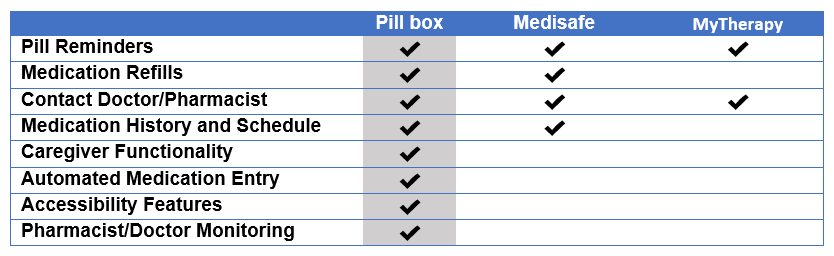
\includegraphics[height=10.5cm]{CompetitiveAdvantage.png}

\end{block}


\begin{block}{Results}
\begin{itemize}
\item 1 week, part of Science Odyssey 2018
\item 408 animations / static graphics created by grade 6-8 classes from 7 schools
\item 5 reading games created by grade 11 and 12 students incorporate those animations
\end{itemize}

\begin{figure}[htbp] %  figure placement: here, top, bottom, or page
\begin{subfigure}{0.49\textwidth}
   \centering
   
\includegraphics[width=19cm]{dh.png}
   \caption*{\textit{Word Direction} game created by high school students in the Wordathon. The animations and pictures were created in parallel by grade 6-8 students and added into the game.}
   \label{fig:TwoAngles}
\end{subfigure}
\begin{subfigure}{0.45\textwidth}
   \centering
   
\includegraphics[width=19cm]{dh.png}
   \caption*{Students develop code using our online code editor and mentoring system.}
   \label{fig:TwoAngles}
\end{subfigure}
\end{figure}


\end{block}

\begin{block}{Conclusions \& Future Work}
The desing allows for medication users, the pharmacist, and caregivers to be involved in the medication process. Pillbox intends on sending out a survery to ensure that nothing was missed in during our requirements gathering. Pillbox is ready to start designing and implementing the solution. We intend on creating the mobile application and having it ready for testing by early 2019. There is always room to improve and adding more features is always up for discussion.

\end{block}

\begin{block}{Acknowledgements}
The Pillbox team would like to thank Dr. Kehdri for all the help and guidance he has done.
\end{block}

\begin{block}{References}
\setbeamertemplate{bibliography item}{\insertbiblabel}
\bibliographystyle{ieeetr}
{\scriptsize
\bibliography{bib}}
\end{block}

\begin{comment}
%these aren't in any particular style, it's just the basic idea
\begin{block}{References}
\setbeamertemplate{bibliography item}{\insertbiblabel}
\bibliographystyle{ieeetr}
{\scriptsize
\bibliography{bib}}
\end{block}
\vspace{-1.8mm}
%will need some more graphics to thank the various people
\end{comment}
\begin{figure}[htbp]
\centering

\includegraphics[height=5cm]{dh.png}
\hspace{1cm}

\includegraphics[height=5cm]{dh.png}
\hspace{1cm}

\includegraphics[height=5cm]{dh.png}
\hspace{1cm}

\includegraphics[height=5cm]{dh.png}
\end{figure}
\end{textblock}

\begin{textblock}{2}(0.44,13.7)

\includegraphics[height=10cm]{dh.png}
\end{textblock}
\begin{textblock}{2}(2.347142857142857,13.7)

\includegraphics[height=10cm]{dh.png}
\end{textblock}
\begin{textblock}{2}(4.2542857142857144,13.7)

\includegraphics[height=10cm]{dh.png}
\end{textblock}
\begin{textblock}{2}(6.161428571428572,13.7)

\includegraphics[height=10cm]{dh.png}
\end{textblock}
\begin{textblock}{2}(8.068571428571428,13.7)

\includegraphics[height=10cm]{dh.png}
\end{textblock}
\begin{textblock}{2}(9.975714285714284,13.7)

\includegraphics[height=10cm]{dh.png}
\end{textblock}
\begin{textblock}{2}(11.882857142857143,13.7)

\includegraphics[height=10cm]{dh.png}
\end{textblock}
\begin{textblock}{2}(13.79,13.7)

\includegraphics[height=10cm]{dh.png}
\end{textblock}

\end{frame}
\end{document}
